\subsection{Evolução do Módulo e Estratégia de Contagem}
\label{subsec:module_evolution}

As etapas descritas anteriormente foram imprescindíveis, para delinear pontos fracos acerca do módulo de contagem de pessoas existente e através da visualização e análise dos dados, compreender como este componente do sistema pode ser evoluído. Sendo assim, a presente subseção pretende apresentar uma sequência de etapas que compõe a nova estratégia utilizada para contagem de indivíduos pelo sistema, que tem como principal objetivo suprir as necessidades destacadas anteriormente, como lidar de melhor forma com a interferência entre os sensores e identificar possíveis eventos de interesse com mais assertividade.

\begin{figure}[H]
    \center
    \fbox{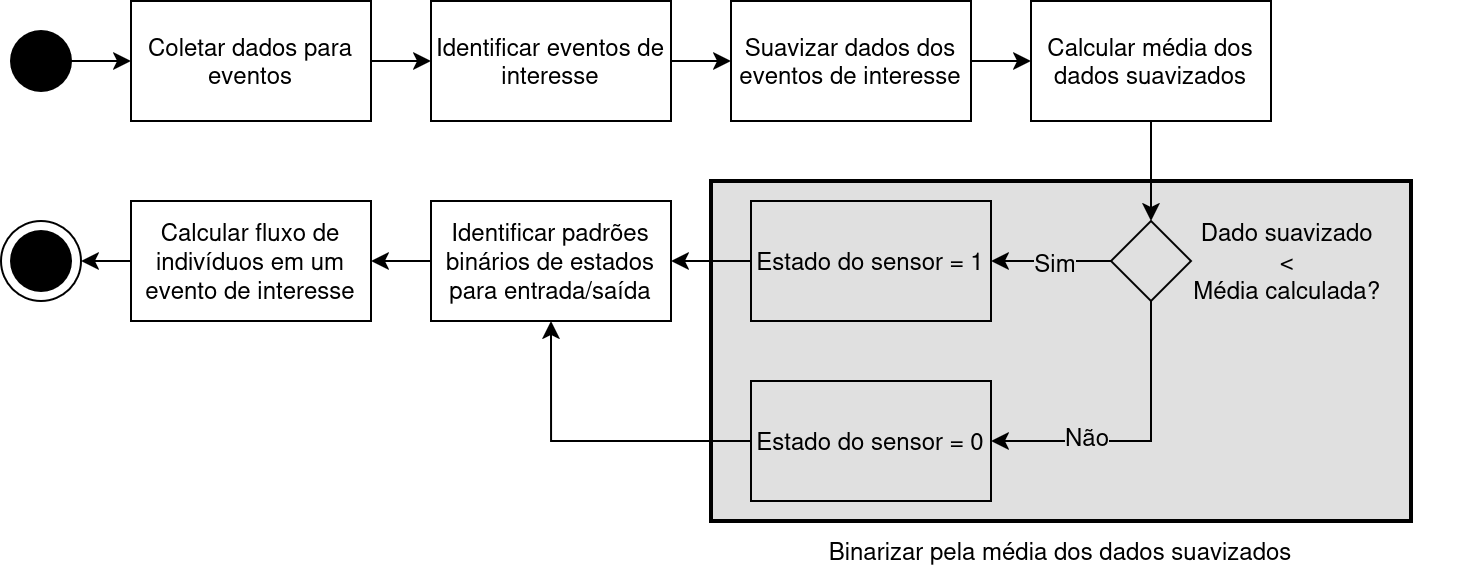
\includegraphics[width=\linewidth]{images/fluxo_new_approach.png}}
    \caption{Fluxo de procedimentos para o cálculo de fluxo de pessoas em um evento}
    \label{fig:strategy_workflow}
\end{figure}

A Figura \ref{fig:strategy_workflow} apresenta de forma sucinta, o fluxo de etapas que compõem o processo de contagem de indivíduos pelo sistema. Em contraste ao Algoritmo \ref{alg:people_counting} pode-se observar a adoção de duas novas etapas de pré-processamento, agregar medidas e suavizar dados coletados. Além disso, a discretização por meio da criação de estados de ativação(ativo ou inativo) foi mantida, no entanto a estratégia para obtenção do limite de binarização foi evoluída, para que esse valor seja obtido de forma dinâmica para cada evento detectado pelo sistema, ou seja, para cada conjunto de dados coletados.

O processo de identificar uma sequência de dados que podem conter um evento de interesse, consiste em uma tarefa difícil como destacado em parágrafos anteriores, mais especificamente delimitar seu início e fim, tendo em vista que a interferência causada entre os sensores gera variações abruptas nos dados coletados, assim como apresentado na Figura \ref{fig:noise_analysis}. Para lidar com este tipo de comportamento, foi adicionado a etapa de agregação de medidas, que consiste apenas na soma das leituras realizadas pelo sensor externo e interno, gerando um novo tipo de informação, que é utilizado para identificar medidas que correspondem há um evento de interesse. A lógica para seu uso é muito simples, durante períodos de inatividade, isto é, que não há nenhum indivíduo entrando ou saindo da instalação, a soma das leituras deve estar compreendida em um intervalo fixo e não deve variar muito. O motivo para este comportamento consiste no fato de que, períodos de inatividade correspondem a observação de eventos estáticos, que por sua natureza  apresentam dados mais regulares, esta característica pode ser observada através dos pontos azuis presentes na Figura \ref{fig:data_collect}. Deste modo, por exclusão, pode-se concluir que apenas medidas que não se encaixam nestes parâmetros podem representar eventos de interesse. Esta abordagem é utilizada para separar e armazenar conjuntos de dados que não necessariamente retratam este tipo de evento, mas que são grandes candidatos para tal.

Mesmo após a identificação de conjuntos de dados que possam conter eventos de interesse, ainda é necessário lidar com problemas causados pela interferência entre os sensores, tendo em vista que, a existência de medidas incorretas pode impedir que o sistema identifique e contabilize uma entrada ou saída. Por este motivo, a próxima etapa após a construção destes conjuntos consiste na suavização dos dados coletados, é possível utilizar esta abordagem, pois o sistema coleta medidas com uma frequência alta, logo por mais que existam dados incorretos, outros pontos em sua vizinhança tem influência acerca do valor daquela medida, impedindo que ela corresponda a valores com grande variação. 

\begin{figure}[H]
    \centering

    % --- Primeira linha ---
    \begin{subfigure}[b]{0.48\textwidth}
        \centering
	    \fbox{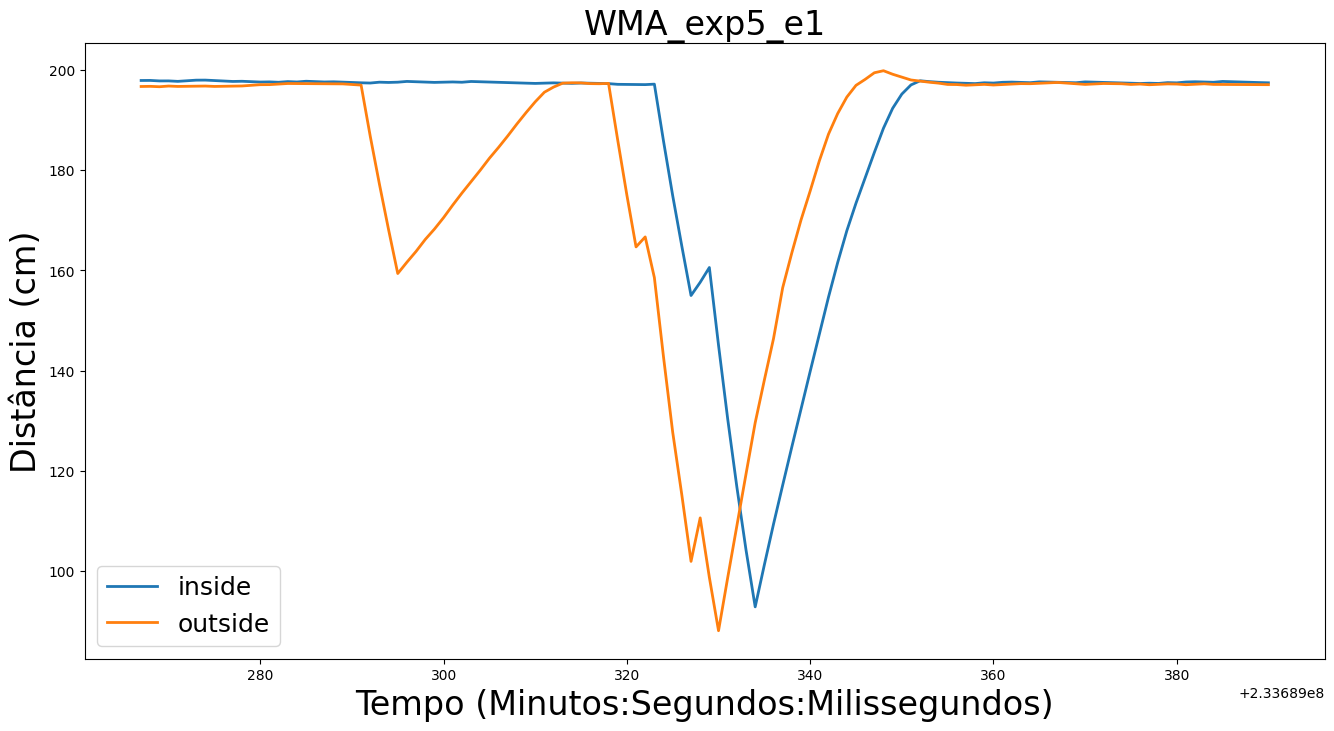
\includegraphics[width=\textwidth]{images/wma_plot.png}}
        \caption{Suavização utilizando Médias Móveis com Peso}
        \label{fig:wma_smooth}
    \end{subfigure}
    \hfill
    \begin{subfigure}[b]{0.48\textwidth}
        \centering
	    \fbox{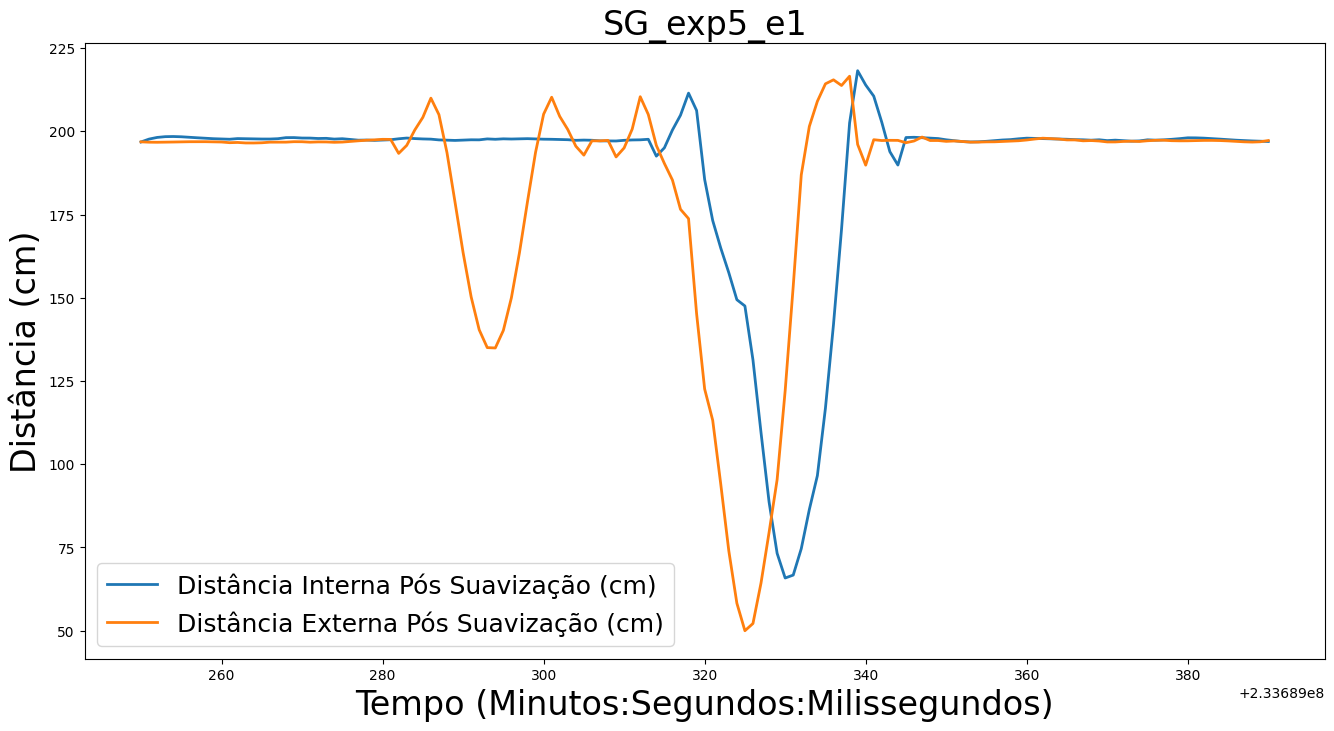
\includegraphics[width=\textwidth]{images/savgol_plot.png}}
        \caption{Suavização utilizando Savitzky-Golay}
        \label{fig:savgol_smooth}
    \end{subfigure}

    \vspace{0.4cm}

    % --- Segunda linha ---
    \begin{subfigure}[b]{0.9\textwidth}
        \centering
	    \fbox{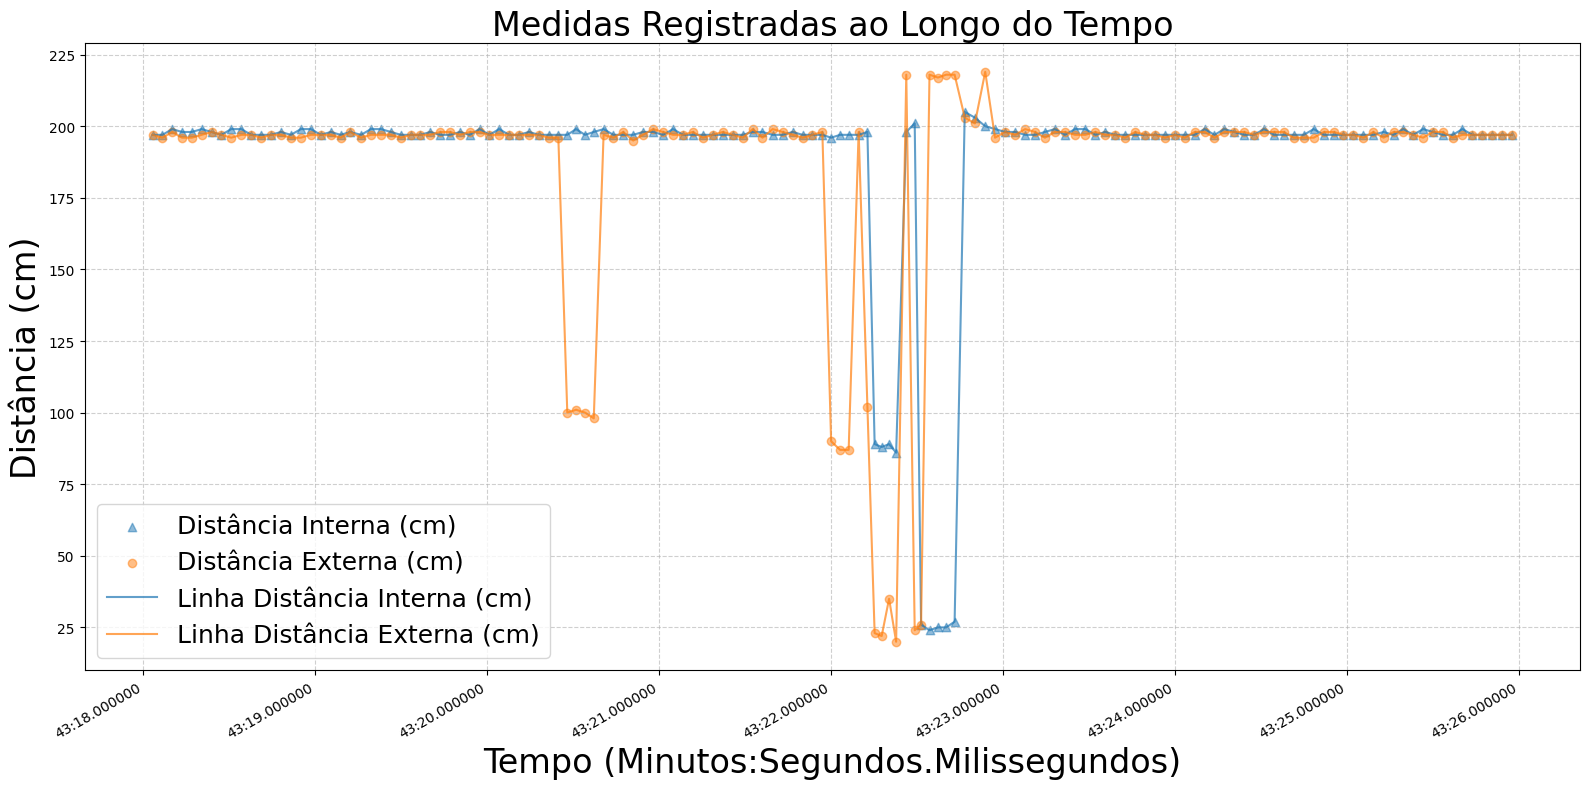
\includegraphics[width=\textwidth]{images/plot_pre_smooth.png}}
        \caption{Apresentação dos dados sem suavização das amostras}
        \label{fig:pre_smooth}
    \end{subfigure}

    \caption{Comparação entre técnicas de suavização de dados aplicadas às medições dos sensores ultrassônicos.}
    \label{fig:smoothing_analysis}
\end{figure}

A Figura \ref{fig:smoothing_analysis} apresenta duas técnicas muito comuns para suavização de dados que possuem ruído e também atenuação de sinal. Neste contexto, a Figura \ref{fig:wma_smooth} corresponde ao emprego de um algoritmo de Média Móveis com Peso (\textit{Weighted Moving Average} - WMA), uma estratégia simples que consiste na ideia de quão maior a distância entre dois pontos, menor a influência entre eles \cite{wang_time_2020}. A equação \ref{eq:wma} apresenta a definição para este tipo de abordagem, neste contexto $\omega_i$ corresponde ao peso/influência da informação presente na posição $i$ acerca do dado contido na posição $t$. Através da Figura \ref{fig:smoothing_analysis}, pode-se observar que esta abordagem gera uma série temporal livre de ruídos e fiel ao comportamento original que pode ser observado na Figura \ref{fig:pre_smooth}. No entanto por não utilizar artifícios polinomiais a representação apresenta picos e variações abruptas, este tipo de comportamento dificulta o processo de caracterização do evento de interesse entre os dados analisados, pois pode gerar falsos positivos durante a etapa de reconhecimento de padrões.

\begin{equation}
\hat{x}_t = \sum_{i=-n}^{n} \omega_i x_{i+t}
\label{eq:wma}
\end{equation}

Outro método muito comum de suavização de dados, mais especificamente no âmbito da engenharia elétrica, consiste no filtro de Savistky-Golay \cite{schafer_what_2011}, que utiliza a ideia de suavização polinomial por mínimos quadrados. Essa técnica consiste em aproximar um conjunto $2M + 1$ de amostras $x[n]$, centradas em $n=0$, por um polinômio $p(n)$ de grau $N$, cujos coeficientes são determinados de modo a minimizar a soma dos erros quadráticos entre o polinômio e as amostras, como apresentado na Equação \ref{eq:erro_sg}. O valor suavizado no ponto central é obtido avaliando o polinômio em $n = 0$, isto é, $y[0]=p[0]=a_0$.

\begin{equation}
\begin{aligned}
\mathcal{E}_N 
&= \sum_{n=-M}^{M} \left( p(n) - x[n] \right)^2 = \sum_{n=-M}^{M} \left( \sum_{k=0}^{N} a_k n^k - x[n] \right)^2
\end{aligned}
\label{eq:erro_sg}
\end{equation}


A Figura~\ref{fig:savgol_smooth} apresenta a aplicação do filtro de Savitzky-Golay ao mesmo conjunto de dados, permitindo a comparação direta com a técnica de WMA. Observa-se que o emprego de técnicas polinomiais resulta em variações mais suaves, algo vantajoso por dois motivos principais. Primeiramente, os vales passam a apresentar formas mais arredondadas e sem variações abruptas, evitando sequências do tipo vale–pico–vale, sem que seja necessário a adoção de uma grande janela de amostras, o que reduz a ocorrência de falsas mudanças no estado de ativação dos sensores e confere maior estabilidade numérica ao sistema. Além disso, nota-se a formação de regiões de decaimento após cada grande vale, o que é particularmente útil, uma vez que a definição dos estados de ativação é realizada por meio da binarização pela média dos valores coletados. Dessa forma, a existência de um tempo de decaimento contribui para uma transição mais suave e confiável entre os estados. Por este motivo, a abordagem adotada para o processo de suavização dos dados no sistema SAFE/UFRJ, foi o filtro de Savistky-Golay.

Após o processo de suavização, é realizado a binarização por limiares para que sejam determinados os estados de ativação dos sensores interno e externo para cada medida coletada. O intuito desta binarização é o mesmo presente no Algoritmo \ref{alg:people_counting}, espera-se que através de uma sequência pré-determinada de estados, seja possível identificar e contabilizar um evento de interesse. No entanto, ao aplicar o filtro de Savistky-Golay o valor numérico coletado pelos sensores é atenuado, deste modo os limites anteriores, valores constantes, não funcionam de forma tão eficaz como anteriormente. Para gerar o novo limite de binarização, é utilizado a Equação \ref{eq:media_geral_compacta}, que consiste na média aritmética entre a média das medidas externas e a média das medidas internas após a aplicação do filtro de Savistky-Golay. 

\begin{equation}
\bar{x}_{geral}
= \frac{1}{2}
\left(
	\frac{1}{N} \sum_{n=1}^{N} x_{externo}[n]
+
	\frac{1}{N} \sum_{n=1}^{N} x_{interno}[n]
\right)
\label{eq:media_geral_compacta}
\end{equation}

O valor obtido por meio da Equação~\ref{eq:media_geral_compacta} pode ser interpretado como uma estimativa do nível médio das medições realizadas pelos dois sensores e pode ser observado através da Figura \ref{fig:smoothing_ex}. Dessa forma, valores inferiores a esse limiar são associados à ativação do sensor, indicando a presença de um indivíduo ou objeto abaixo do sensor, enquanto valores superiores correspondem a inatividade. Com o objetivo de evitar ativações indevidas causadas por objetos de pequenas dimensões ou ruídos de medição, foi estabelecido um limite mínimo adicional de 50~cm, determinado de forma experimental.

\begin{figure}[H]
    \centering

    % --- Primeira linha ---
    \begin{subfigure}[b]{0.48\textwidth}
        \centering
	    \fbox{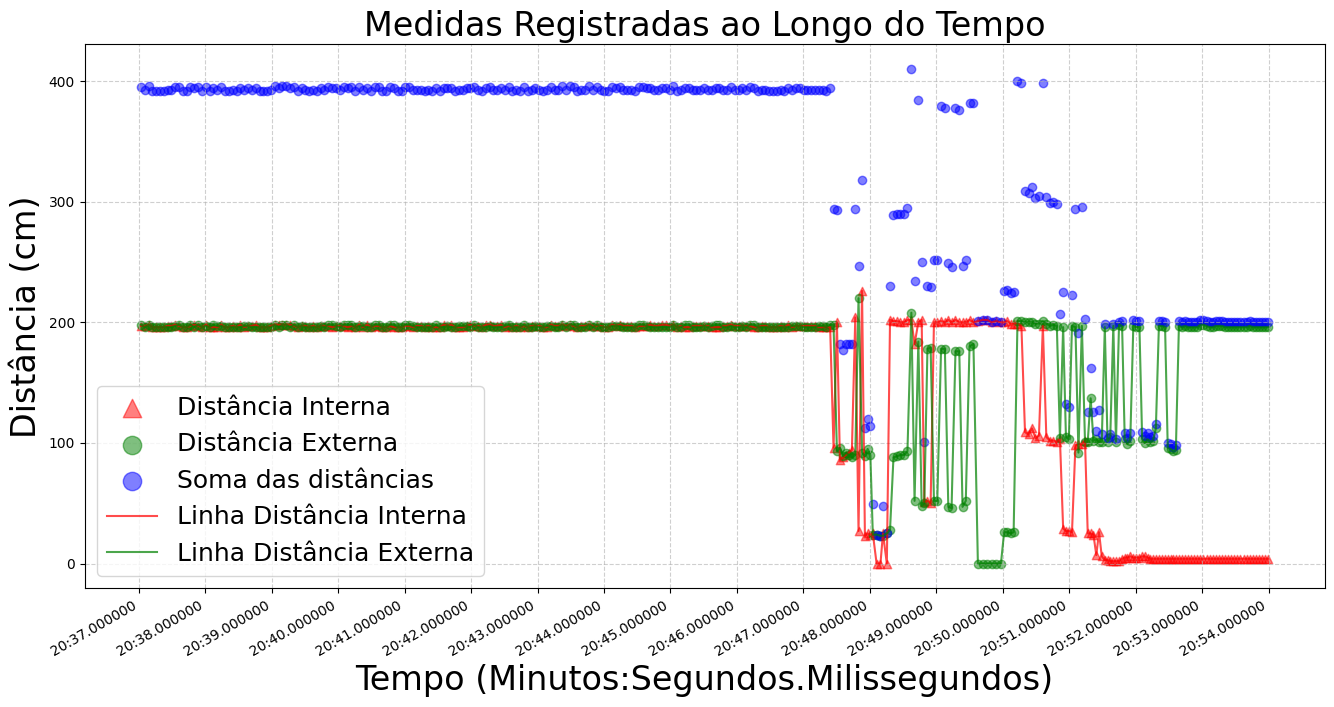
\includegraphics[width=\textwidth]{images/plot_event_ex.png}}
        \caption{Janela temporal de medidas coletadas}
        \label{fig:plot_ex}
    \end{subfigure}
    \hfill
    \begin{subfigure}[b]{0.48\textwidth}
        \centering
	    \fbox{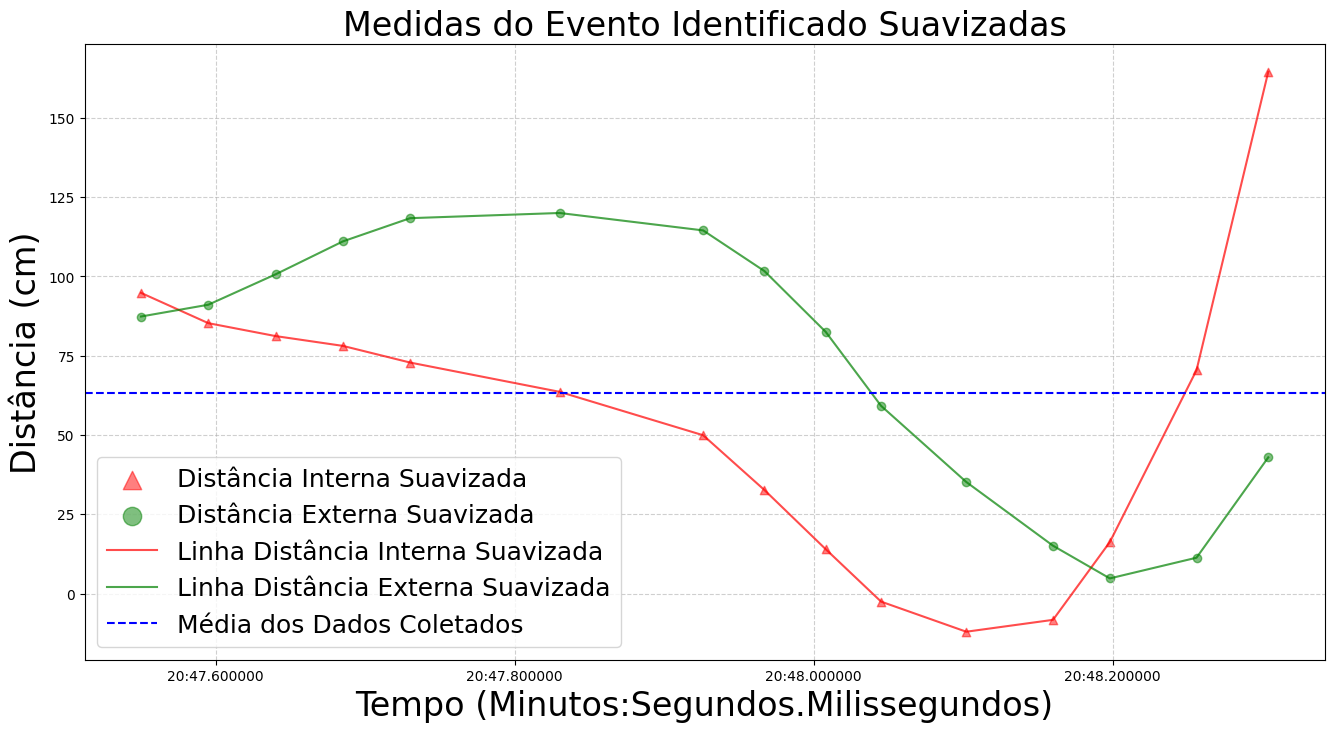
\includegraphics[width=\textwidth]{images/smoothing_ex.png}}
        \caption{Suavização das medidas de um evento}
        \label{fig:smoothing_ex}
    \end{subfigure}

    \vspace{0.4cm}

    % --- Segunda linha ---
    \begin{subfigure}[b]{0.9\textwidth}
        \centering
	    \fbox{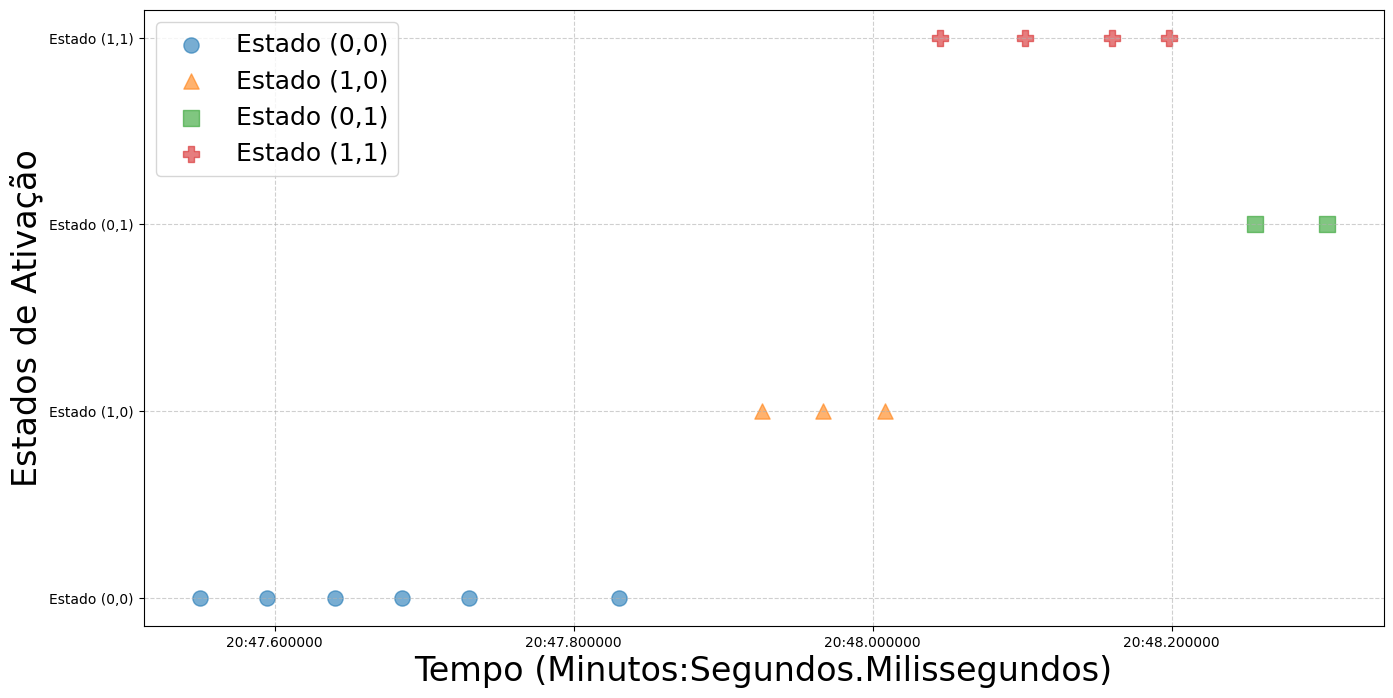
\includegraphics[width=\textwidth]{images/binarization_ex.png}}
        \caption{Estados de ativação para cada medida do evento}
        \label{fig:bin_ex}
    \end{subfigure}

    \caption{Processo de obtenção dos estados de ativação dos sensores desde a coleta de dados.}
    \label{fig:entire_cicle_ex}
\end{figure}

Após o processo de binarização disposto na Figura \ref{fig:entire_cicle_ex}, espera-se obter um conjunto de dados que permita identificar através de valores binários (0 e 1), qual a ordem de acionamento dos sensores durante possíveis eventos de interesse. Para este processo de identificação, é necessário realizar a junção dos valores binários correspondentes ao sensor externo e interno para cada medida, obtendo-se uma tupla denominada como estado de ativação do módulo de sensoriamento, assim como disposto na Figura \ref{fig:bin_ex}. Desta forma, ao identificar todos os estados de ativação que compõem o evento, bem como a ordem em que eles ocorrem, torna-se possível caracterizar o evento em uma entrada ou saída. Esse processo está descrito como Caracterização do Evento de Interesse na Figura \ref{fig:strategy_workflow} e faz uso da Tabela \ref{tab:state_machine} como modelo para análise dos eventos.

\begin{table}[H]
	\centering
	\caption{Transição de Estados do Módulo de Contagem de Pessoas}\label{tab:state_machine}
	\begin{tabular}{|c|c|c|l|}
		\hline
		\multicolumn{1}{|l|}{\textbf{Estado Inicial}} & \multicolumn{1}{l|}{\textbf{Estado Final}} & \textbf{Transições de Estados}                & \multicolumn{1}{c|}{\textbf{Descrição do evento}} \\ \hline
		(1,0)                                         & (0,1)                                      & (1,0) -\textgreater (1,1) -\textgreater (0,1) & Alguém entrou                                     \\ \hline
		(0,1)                                         & (1,0)                                      & (0,1) -\textgreater (1,1) -\textgreater (1,0) & Alguém saiu                                       \\ \hline
	\end{tabular}
\end{table}

Por fim, a etapa de caracterização consiste em analisar a sequência de estados de ativação gerada e buscar por conjuntos com ordem de acontecimentos bem definida, assim como apresentado na coluna de Transições de Estado através da Figura \ref{tab:state_machine}. Como espera-se que o algoritmo seja capaz de filtrar momentos de inatividade, o modelo utilizado para caracterizar eventos registrados não contém o estado (0,0), que corresponde a inatividade dos dois sensores ultrassônicos. Além disso, graças ao processo de suavização das medidas coletadas, caso de fato ocorra uma entrada ou saída, os valores tendem a transicionar de um estado de ativação para o outro de forma mais suave, logo o estado de ativação (1,1), que corresponde a ativação de ambos os sensores, sempre deve ocorrer, se tornando um estado ativação em comum entre os dois eventos e essencial para eventos válidos.


